

\documentclass[]{scrartcl}

\usepackage{graphicx}
%\graphicspath{ {./images/} }

%opening
\title{Artificial Intelligence and Machine Learning Engineer}
\author{Chanh Huan Tran}

\begin{document}

\maketitle

\begin{abstract}
This is a look at two sample problems in AI ML.

\end{abstract}

\section{Basketball Probability Model}
%\includegraphics{universe}
\section{Anomaly Detection Model}

This section will introduce techniques to determine an anomaly.

Below is a table of widths and heights (in pixels) belonging to different figures:

Width
Height
25
24
25
25
25
25
21
24
24
24
30
29
25
25
25
25
27
29
25
29
24
29
24
25
27
25
24
27
24
25
25
24
24
25
25
30
29
29
27
30
27
24
29
25
27
25
25
25
23
29

Using a machine learning algorithm, can you determine if a figure with width 30 and height 22 is considered an anomaly in the above data set?

% TODO: \usepackage{graphicx} required
\begin{figure}
	\centering
	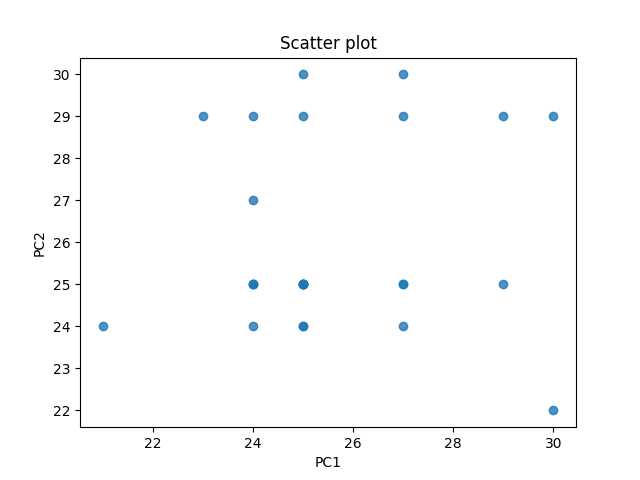
\includegraphics[width=0.7\linewidth]{Figure_1}
	\caption[Anomaly Detection Scatter Plot]{Take a look at the landscape.}
	\label{fig:figure1}
\end{figure}

\begin{figure}
	\centering
	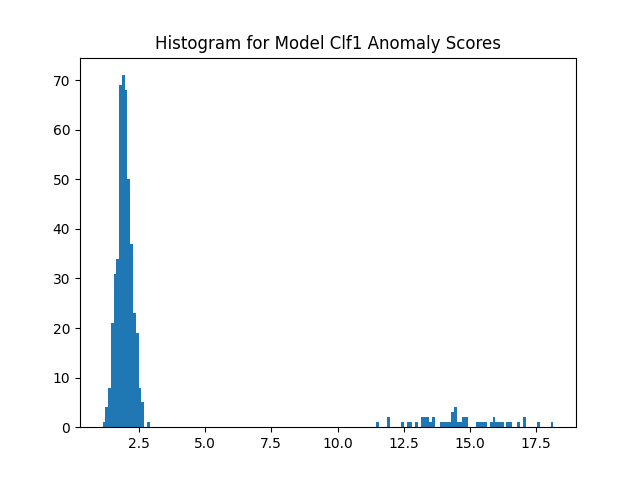
\includegraphics[width=0.7\linewidth]{Figure_2}
	\caption[Anomaly Detection Histogram]{Iterative approach to developing artificial intelligence algorithm.}
	\label{fig:figure2}
\end{figure}

\begin{figure}
	\centering
	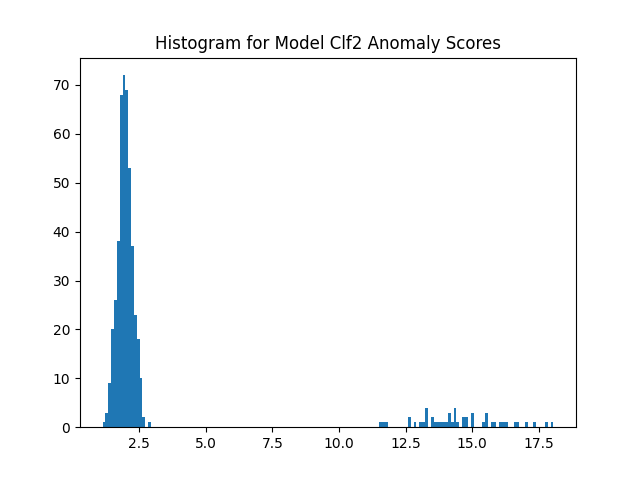
\includegraphics[width=0.7\linewidth]{Figure_3}
	\caption[Anomaly Detection Histogram]{Iterative approach to developing artificial intelligence algorithm.}
	\label{fig:figure3}
\end{figure}

\begin{figure}
	\centering
	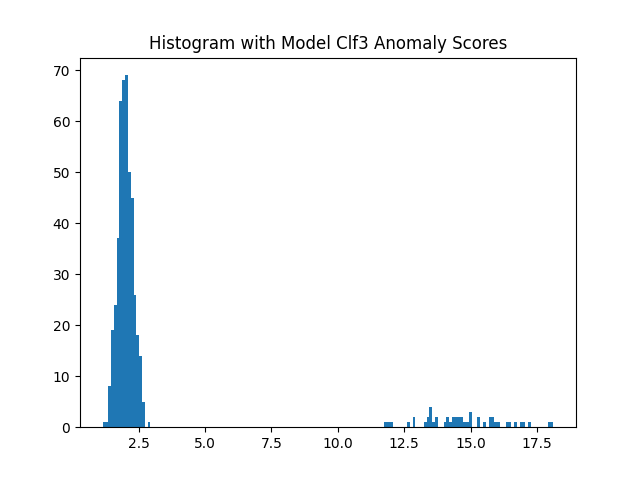
\includegraphics[width=0.7\linewidth]{Figure_4}
	\caption[Anomaly Detection Histogram]{Iterative approach to developing artificial intelligence algorithm.}
	\label{fig:figure4}
\end{figure}


\end{document}
